\begin{tikzpicture}
	\draw (0,0) -- node[midway, below] {$ \dfrac{1}{\alpha T} $} (4.1,0);
	
	\draw (0,0) -- (45:3.67);
	
	\draw (0.5,0) arc (0:45:0.5) node[midway, right, yshift=2pt] {$ \ang{45} $};
	
	\draw (4.1,0) -- +(120:3) node[midway,right] {$ \omega_n $};
	
	\draw (3.6,0) arc (180:120:0.5) node[midway, left, yshift=2pt] {$ \theta $};
	
	\draw (2.6,2.6) +(-0.35,-0.35) arc (225:300:0.5) node[coordinate, name=C] {};
	
	\draw[->] (C) +(-0.2,0.1) parabola bend (2.5,2.4) (2.3,2.6) node[above] {$ \dfrac{\ang{180}-\theta}{2}+\dfrac{\phi}{2}=\ang{75} $};
\end{tikzpicture}